\section{Results}
\label{sec:results}

For the first part of the experiment we simply run all the different classification methods explained in Section~\ref{sec:setup} randomly splitting the dataset into $70\%$ training and $30\%$ testing. The results can be clearly seen in Tab.~\ref{tab:singleChordResults}.

\begin{table}[t]
\centering
\begin{tabular}{|c|c|c|c|}
	\hline
	& CLP & CENS & CRP \\
	\hline
	GMM & 14.58\% & 6.94\% & 11.81\% \\
	\hline
	SVM (linear) & 13.61\% & 6.39\% & 12.64\% \\
	\hline
	SVM (poly) & 10.56\% & 4.17\% & 7.92\% \\
	\hline
	SVM (RBF) & 10.00\% & 4.31\% & 7.78\% \\
	\hline
\end{tabular}
\caption{Results of the first part of the tests (single chord recognition).}
\label{tab:singleChordResults}
\end{table}


As said in the previous section, in the second part of the experiment we got two different kind of outputs, which are $\mathcal{L}_{SVM}$ and $\mathcal{L}_{HMM}$. In order to verify the quality of ours results we compared them with  $\mathcal{L}_{Harte}$. Given $\mathcal{L}_{SVM}$ ($\mathcal{L}_{HMM}$) and $\mathcal{L}_{Harte}$ for a certain value of $r_{test}$ and for a certain extracted feature we computed the error probability doing the ratio between all the matching between $\mathcal{L}_{SVM}$ ($\mathcal{L}_{HMM}$) and $\mathcal{L}_{Harte}$.

 In Tab.~\ref{tab:resultbeforeHMM} we can look at the error probabilities obtained after the first step of testing, therefore before processing HMM. In Tab.~\ref{tab:resultafterHMM} we can look at the results obtained after the second step of testing, therefore after processing HMM. In both cases we have different outputs depending on the testing rate $r_{test}$ and on the chosen extracted feature.

\begin{table}[h!]
	\caption{Results of the second part before processing HMM}
	\centering
	\begin{tabular}{|c |c c c|}
	\hline
	$r_{test}$ & CENS & CLP & CRP\\ \hline
	0.1 & 0.4946 & 0.4739 & 0.6206\\
	0.2 & 0.4657 & 0.6000 & 0.6376\\
	0.3 & 0.4765 & 0.5691 & 0.5803\\
	\hline
	\end{tabular}
	\label{tab:resultbeforeHMM}
\end{table}

\begin{table}[h!]
	\caption{Results of the second parts after processing HMM}
	\centering
	\begin{tabular}{|c |c c c|}
	\hline
	$r_{test}$ & CENS & CLP & CRP\\ \hline
	0.1 & 0.4439 & 0.4502 & 0.5641\\
	0.2 & 0.4296 & 0.5919 & 0.5967\\
	0.3 & 0.4179 & 0.5484 & 0.5204\\
	\hline
	\end{tabular}
	\label{tab:resultafterHMM}
\end{table}

 Observing the results we can state what follows. First, we got best results with CENS features than with CLP and CRP features. We explain this remembering that in order to keep low the computational cost of our setup, we strongly limited the features extraction for CLP and CRP. Second, HMM proved to be able to enhance better results than MC-SVM alone. This is not obvious since we worked with features of multi-instrumental sounds which also include vocal parts. Indeed the chords prediction of some songs often isn't improved bu aggravated. We can show this by comparing the two different results obtained with the same $\mathcal{D}_{train}$ as done in Fig.~\ref{fig:compareerror}.

\begin{figure} [h!]
	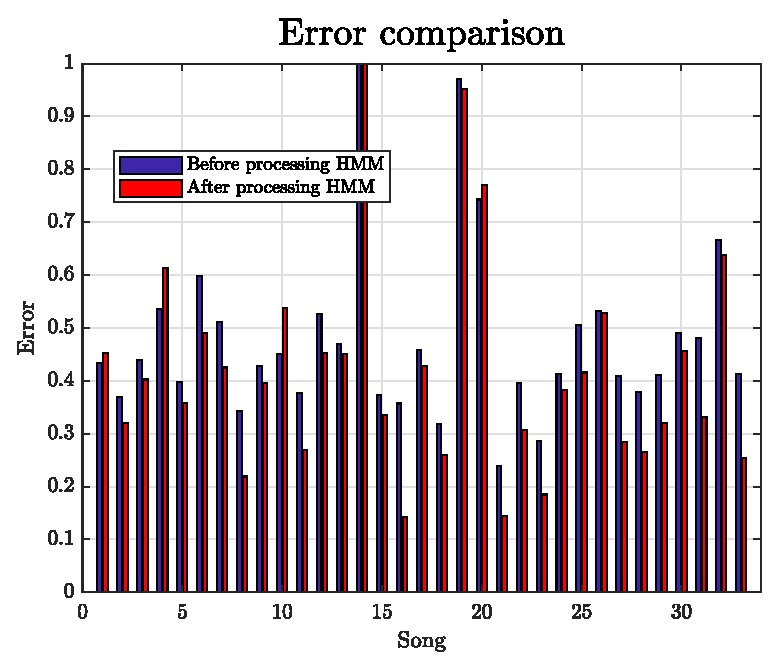
\includegraphics[width=0.5\textwidth]{img/Result_HMM/CENS/plot03071}
	\caption{Error comparison using CENS features and $r_{test}=0.3$}
	\label{fig:copareerror}
\end{figure}

We concluded that HMM isn't always improving our result for every single song. It is able to do so only in average. However what HMM is doing for each song is reduce the chords variation, that is the number of times that a chord varies within the same song. This happens since HMM tends to correct most improbables outputs generated by MC-SVM. We find confirmation to ours assumption looking at
Fig.~\ref{fig:smoothmulti} and Fig.~\ref{fig:smoothsingle}.

\begin{figure} [h!]
	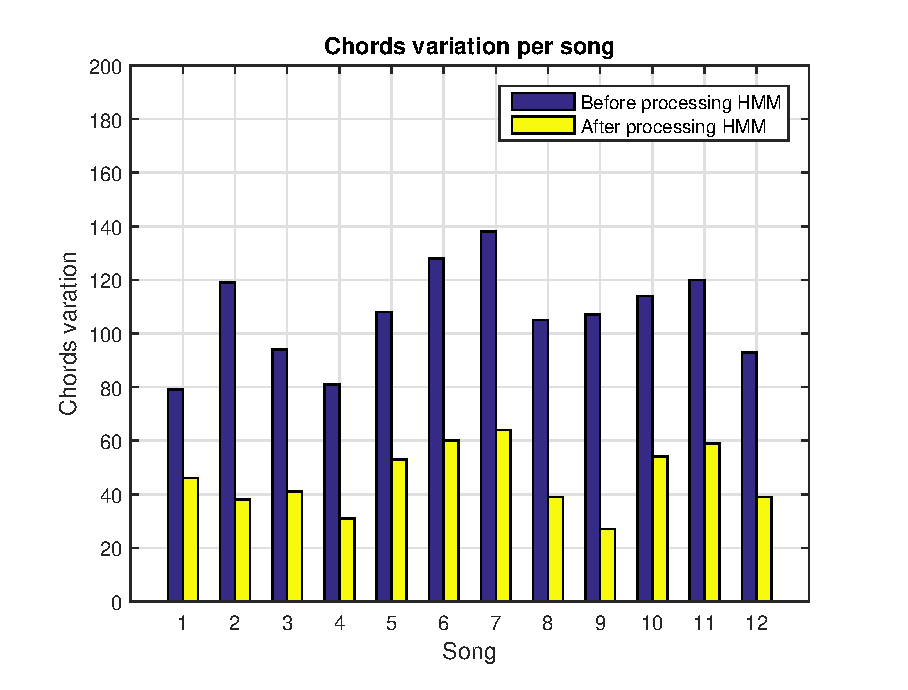
\includegraphics[width=0.5\textwidth]{img/Result_HMM/SMOOTHING/SmoothPerSongCENS0109}
	\caption{Chords variation per song using CENS features and $r_{test}=0.1$}
	\label{fig:smoothmulti}
\end{figure}

\begin{figure} [h!]
	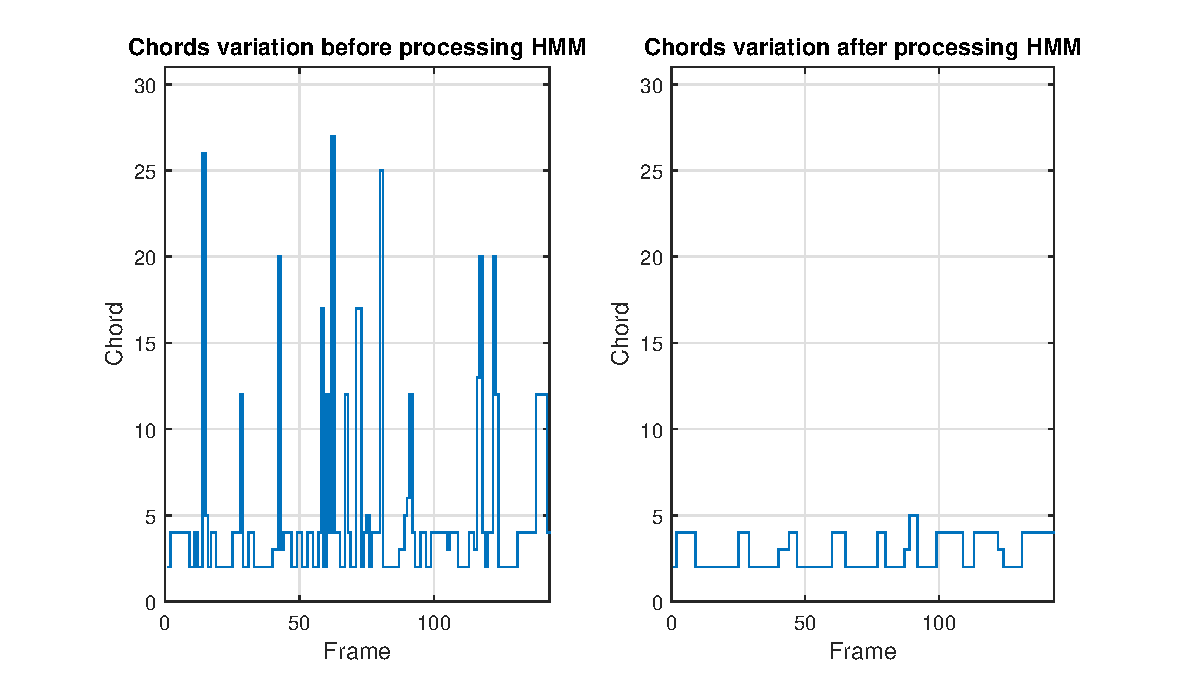
\includegraphics[width=0.5\textwidth]{img/Result_HMM/SMOOTHING/SmoothSingleSongCENS0109}
	\caption{Chord variation in a single song using CENS features and $r_{test}=0.1$}
	\label{fig:smoothsingle}
\end{figure}
